\documentclass[12pt]{article}\usepackage[]{graphicx}\usepackage[]{color}
%% maxwidth is the original width if it is less than linewidth
%% otherwise use linewidth (to make sure the graphics do not exceed the margin)
\makeatletter
\def\maxwidth{ %
  \ifdim\Gin@nat@width>\linewidth
    \linewidth
  \else
    \Gin@nat@width
  \fi
}
\makeatother

\definecolor{fgcolor}{rgb}{0.345, 0.345, 0.345}
\newcommand{\hlnum}[1]{\textcolor[rgb]{0.686,0.059,0.569}{#1}}%
\newcommand{\hlstr}[1]{\textcolor[rgb]{0.192,0.494,0.8}{#1}}%
\newcommand{\hlcom}[1]{\textcolor[rgb]{0.678,0.584,0.686}{\textit{#1}}}%
\newcommand{\hlopt}[1]{\textcolor[rgb]{0,0,0}{#1}}%
\newcommand{\hlstd}[1]{\textcolor[rgb]{0.345,0.345,0.345}{#1}}%
\newcommand{\hlkwa}[1]{\textcolor[rgb]{0.161,0.373,0.58}{\textbf{#1}}}%
\newcommand{\hlkwb}[1]{\textcolor[rgb]{0.69,0.353,0.396}{#1}}%
\newcommand{\hlkwc}[1]{\textcolor[rgb]{0.333,0.667,0.333}{#1}}%
\newcommand{\hlkwd}[1]{\textcolor[rgb]{0.737,0.353,0.396}{\textbf{#1}}}%
\let\hlipl\hlkwb

\usepackage{framed}
\makeatletter
\newenvironment{kframe}{%
 \def\at@end@of@kframe{}%
 \ifinner\ifhmode%
  \def\at@end@of@kframe{\end{minipage}}%
  \begin{minipage}{\columnwidth}%
 \fi\fi%
 \def\FrameCommand##1{\hskip\@totalleftmargin \hskip-\fboxsep
 \colorbox{shadecolor}{##1}\hskip-\fboxsep
     % There is no \\@totalrightmargin, so:
     \hskip-\linewidth \hskip-\@totalleftmargin \hskip\columnwidth}%
 \MakeFramed {\advance\hsize-\width
   \@totalleftmargin\z@ \linewidth\hsize
   \@setminipage}}%
 {\par\unskip\endMakeFramed%
 \at@end@of@kframe}
\makeatother

\definecolor{shadecolor}{rgb}{.97, .97, .97}
\definecolor{messagecolor}{rgb}{0, 0, 0}
\definecolor{warningcolor}{rgb}{1, 0, 1}
\definecolor{errorcolor}{rgb}{1, 0, 0}
\newenvironment{knitrout}{}{} % an empty environment to be redefined in TeX

\usepackage{alltt}

%\usepackage[roman]{../pres1}
%\usepackage[sans]{../pres1}

\usepackage[hmargin=1in,vmargin=1in]{geometry}
\usepackage{parskip}
\usepackage{hyperref}
\usepackage{graphicx}
\usepackage{color}
\hypersetup{pdfstartview=FitV,hidelinks}
\IfFileExists{upquote.sty}{\usepackage{upquote}}{}
\begin{document}

{
  \Large
  \centering
  Lab 8 Assignment --- Occupancy Models \\
  Due before your next lab \par
}

\vspace{10pt}

%% Answer each of the following questions and upload your answers to ELC
%% as a single Excel file. Be sure to show your calculations. Name the
%% file something like: \texttt{Chandler\_Richard-lab8.xlsx}. \\

Answer each of the following questions, and submit your answers by
uploading a single \textcolor{red}{WORD} file to ELC. Unlike previous labs,
copy and paste results from Excel and PRESENCE to the WORD file, or
copy and paste entire screenshots to show the relevant output. Name
the file something like \texttt{Chandler-lab8.docx}.  


%\vspace{12pt}

\section*{\normalsize Preliminaries: Getting Data into Program PRESENCE}
\vspace{-10pt}
\begin{enumerate}
  \itemsep-6pt
  \item[(1)]  Open PRESENCE
  \item[(2)]  Go to \texttt{File > New Project}
  \item[(3)]  Select \texttt{Input Data Form}
  \item[(4)]  Specify the number of rows (sites), columns
    (occasions), and (for Exercise I) the number of site covariates. 
  \item[(5)]  Fill in the number of occasions per season
    (No. Occ/season). For Exercise II, this is the number of teams per
    year. 
  \item[(6)]  Copy and paste occupancy data from Excel into the
    PRESENCE spreadsheet. 
  \item[(7)]  If you have a site covariate, click the \texttt{Site
      Covars} tab and copy and paste the covariate values (and the
    covariate name in the first row) using the option \texttt{Edit > Paste
    w/covnames}.  
  \item[(8)]  Use \texttt{File > Save As} to save the project
    somewhere on your computer. Save it to \texttt{Documents} or
    another location that isn't restricted. Click \texttt{No} when it
    asks if you want to use the last column as frequencies. 
  \item[(9)]  Close the PRESENCE spreadsheet, and click \texttt{OK} on
    the project information window.  
\end{enumerate}


\begin{figure}[h!]
  \centering
  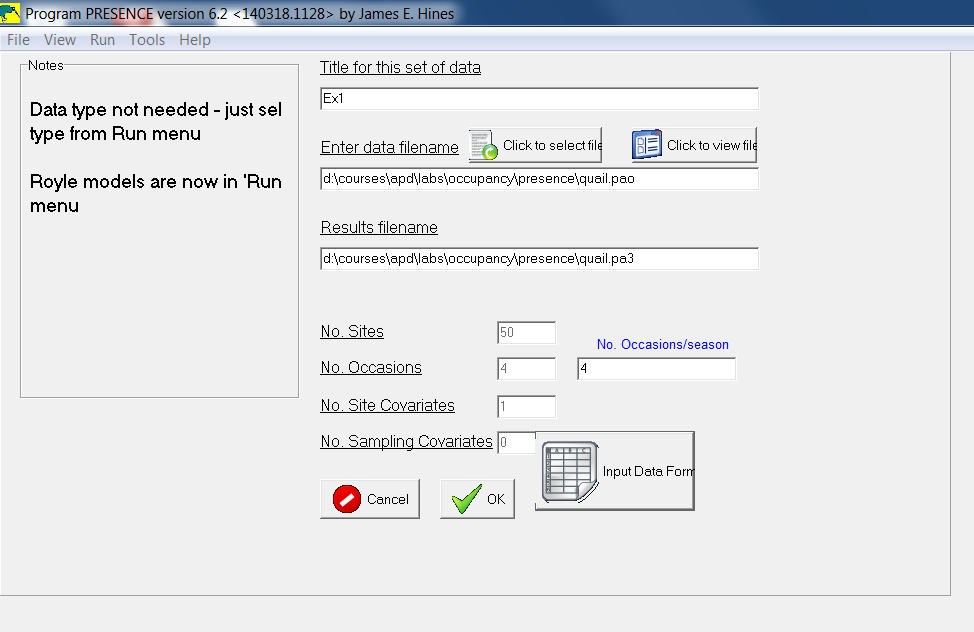
\includegraphics[width=0.7\textwidth]{figs/pres-setup}
  \caption{\small This is where you tell PRESENCE about your data}
  \label{fig:pres-setup}
\end{figure}

\clearpage

\section*{Exercise I: Single-season models}

Suppose we are interested in estimating occupancy of bobwhite quail
({\it Colinus virginianus}) in abandoned ag fields. We randomly select
50 sites and survey them 4 times each May. The resulting data indicate
whether at least one quail was detected at each site on each visit in
each season.    

In addition, you think there is a possibility that vegetation height
affects both occupancy and detection probability so you measure
average vegetation height at each site. Vegetation height will be the
covariate used in the analysis. 

Create a new PRESENCE project and import the quail data. You will
need to specify that there are 50 rows, 4 columns, 4 Occ/season, and 1
site covariate: \texttt{veght}. Make sure you use \texttt{Paste with
  covname} when adding the \texttt{veght} site covariate (see
instructions above).  

\begin{enumerate}
  \item[(a)] Run the single-season analysis without changing the
    defaults (\texttt{Run > Analysis:single-season}). Report the
    estimates and standard errors for psi ($\psi$) and p. Interpret
    these estimates (ie, what are the definitions of psi and p in this
    context?). These can be found by right-clicking on the name of the
    model (which will be something like \texttt{1 group, constant P}
    and clicking on \texttt{View model output}.  There is LOTS of
    output. You want to focus on the \texttt{Individual Site
      Estimates}, which should look something like this: 

\begin{figure}[h!]
  \centering
  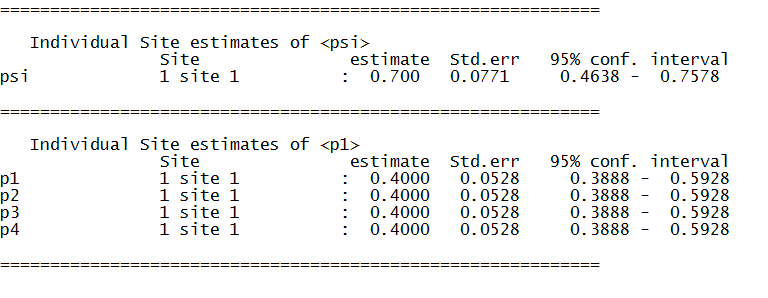
\includegraphics[width=0.9\textwidth]{figs/pres-est}
  \caption{\small Estimates, standard errors, and confidence intervals
  for psi ($\psi$) and $p$.}
  \label{fig:pres-est}
\end{figure}
    
  \item[(b)] Now run another model using \texttt{veght} as a
    predictor variable (covariate). This is tricky. First, choose 
    \texttt{Run > Analysis:single-season}. Then, click on
    \texttt{Custom}, which will open up the ``design matrix''. Now
    right click to \texttt{Add col} on the Occupancy tab (see
    Fig. below). Next, click the cell under \texttt{a2} and select 
    \texttt{Init > *veght} to indicate that you want to model psi
    as a function of vegetation height. Do the same thing under the
    \texttt{Detection} tab, but note that there are multiple rows for
    a1 and a2 this time. Make sure the first column of each matrix has
    1's not 0's (see screenshots below). Close the design matrix
    window and then name the model something like 
    \texttt{psi(veght)p(veght)} and hit \texttt{OK to Run}. 

\begin{figure}[h!]
  \centering
  \fbox{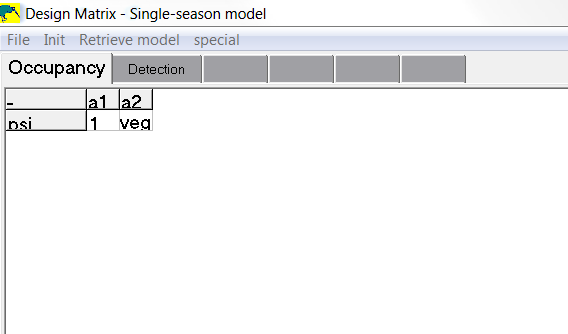
\includegraphics[height=5cm]{figs/pres-des-psi}} \hfill
  \fbox{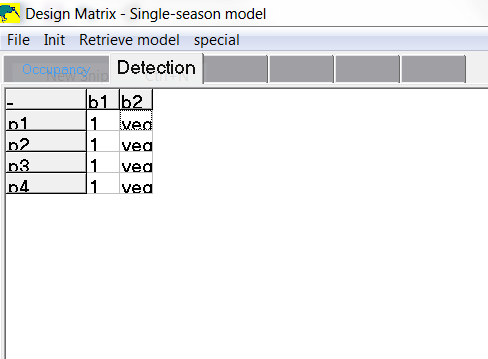
\includegraphics[height=5cm]{figs/pres-des-p}}   \\
  \caption{\small This is where you tell PRESENCE about the covariates
    in the model.}
  \label{fig:pres-design}
\end{figure}
%\clearpage

  \item[(c)] Is this model better than the first, based on AIC? The
    lower the AIC the better the model.\footnote{$\mathrm{AIC} =
      -2*\mathrm{log(likelihood)} + 2*\mathrm{nParameters}$. AIC
      favors models that explain a lot of variation in the data using
      a small number of parameters.}  
  \item[(d)] Right-click on the model and choose 
    \texttt{View model output} to find the parameter estimates under
    \texttt{Untransformed Estimates of coefficients for covariates
      (Beta's)}.  The estimate \texttt{A1} is the estimate of the
    intercept, and \texttt{A2} is the slope parameter defining the
    relationship between psi and vegetation height on the logit
    scale. Use these estimates to create a plot of the relationship
    between occurrence probability and vegetation height. The Excel
    sheet has a template for you to fill in. Add the graph to your
    Word document.
  \item[(e)] Based on your graph, does occurrence probability
    increase or decrease with vegetation height?  
\end{enumerate}

\clearpage

\section*{Exercise II: Multi-season model}

Use the southern two-lined salamander ({\it Eurycea cirrigera})
%Eastern newt ({\it Notophthalmus viridescens}) 
data from the
past few years to do the following. Note: I pooled the data from
the 5 swipes of each team.   

\begin{enumerate}
  \item[(a)] Close your old project, restart PRESENCE, and create a
    new project by importing the salamander
    data. You will need to indicate that there are 15 sites, 35
    columns, and \textcolor{red}{7 occasions per season}. The last piece of
    information tells PRESENCE that there were 5 seasons (with 7 team
    surveys per season).  
  \item[(b)] Use Program PRESENCE to estimate psi ($\psi$), gamma
    ($\gamma$), epsilon ($\epsilon$),
    and p (\texttt{Run > Analysis:multi-season > simple multi-season}
    and accept default settings). The estimates can be found by right clicking on the
    model name and choosing \texttt{View model output}. Look for the 
    \texttt{Real parameter estimates}. Report the 4 unique
    estimates and standard errors by creating a table in your Word
    document.  
  \item[(c)] Provide clear interpretations of your estimates. 
  \item[(d)] Based on these estimates, is there any reason to believe
    that occupancy has decreased over these years? Explain. 
  \item[(e)] How certain are you of these conclusions? Answer by
    describing how well you think our study design met the assumptions
    of the multi-season occupancy model. 

\end{enumerate}




%% \clearpage

%% \section*{Occupancy modeling in \texttt{R}}


%% Occupancy models can be fit using the 'unmarked' package in {\tt R}. 



\end{document}




